\section{Stockholm --- Stockholm Congestion Tax}

% The next city to implement DRP was Stockholm. The Stockholm Congestion Tax has a larger literature than any of the other schemes we cover, due partly to the government's transparency and partly to a proliferation of research by 

\subsection{History}

Discussion of downtown pricing in Stockholm started in the 1980s, with a proposal that cars have to display a transit pass in their windshields \citep{GullbergIsaksson2009,Arnott2005}. In 1989, the City of Stockholm formulated plans for this ``car card'' proposal as well as an electronic cordon pricing system \citep[p. 90]{Hau1992}; but since road pricing was deemed a ``tax'' rather than a ``charge,'' Swedish law required that the national parliament approve it. Despite Stockholm's support, parliament tabled the tax for complex political reasons \citep{Ahlstrand2001}. 

Meanwhile, recognizing that congestion had become serious, the national government convened Stockholm's political parties to negotiate an infrastructure package. The resulting agreement, finalized in 1992 and called the ``Dennis Package,'' resembled the Norwegian toll ring model: tolls in a cordon around central Stockholm would pay for massive highway and tunnel projects designed to keep cars out of central Stockholm (see \citet[pp. 39-40]{Gomez-Ibanez1994} and \citet[p. 92]{Hau1992}). However, in 1997 the government cancelled the Dennis Package due, as before, to complex political maneuverings \citep{Ahlstrand2001,GullbergIsaksson2009}.

In 2000, the Swedish parliament set up a ``Stockholm Commission'' to  prioritize infrastructure projects, and in March 2002 the Commission was directed to reconsider road pricing as a way to pay for them \citep{Eliasson2009b}. As it happened, 2002 was also an election year, and the Moderate Party (Sweden's mainstream conservative party) pounced on the renewed discussion of pricing to win some voters from their rivals, the Social Democrats. In response, a local Social Democrat leader, Annika Billstr\"om, announced on television, ``My message to the voters of Stockholm is that there will be no road charging during our next term of office'' \citep{GullbergIsaksson2009}.

The September 2002 election wound up with the Social Democrats and their allies, the Left Party, just short of a majority both nationally and in Stockholm. Seizing the opportunity, the environmentalist Green Party made a pact to join the Social Democrat's coallition in exchange for a trial of pricing in Stockholm. The deal sparked a public outcry over Annika Billstr\"om's (by then Mayor of Stockholm) broken pledge, and opponents demanded that the decision of whether to instate pricing permanently be made via referendum. The Social Democrats agreed a referendum would follow the trial's conclusion and appear on the September 2006 election ballot. Originally, the trial was meant to last several years, but political and legal complications delayed the start until January 3, 2006. The trial lasted until July 31, 2006.

Prior to the trial, media coverage of the trial was very negative, and polls showed strong opposition. But once the trial began, public opinion shifted quickly in favor due to very visible congestion reductions.\footnote{A small literature now exists on the question of why public opinion shifted---e.g., XXX LIST SOURCES} At the September 2006 elections, 53\% of Stockholm residents voted to make the scheme permanent. However, at the same election, the leftist coalition lost control of the government at all levels to a center-right alliance of parties who opposed pricing---thus throwing the SCT's future into doubt.  But in the end the new government agreed to respect the referendum results after negotiating a \euro 10 billion infrastructure package, whereby toll revenues were matched by national funds to build new roads---as in the Dennis Package. The SCT returned on a permanent basis on August 1, 2007.

\subsection{Design}

The Stockholm Congestion Tax (SCT) is a time-variable toll on weekday trips both into and out of a cordon around central Stockholm. See Fig. \ref{fig:stockholm-map} for a map of the tolling sites, which are mostly unchanged. The map has labeled a highway called the Essingeleden; this was originally toll-free for political reasons---being the only north-south route around the city---but in January 2016, tolls were added to the Essingeleden.

During the trial, the SCT used a radio-frequency tag-and-beacon system backed up by ANPR cameras, but with time the error rate for ANPR became low enough that transponder enforcement was ended in late 2008 \citep[p. 841]{Hamilton2011}. Vehicles are charged when they cross under metal gantries, which work as a trio: when a laser on the middle gantry detects a vehicle, cameras mounted on the first and third photograph the front and rear plates.\footnote{``Frequently asked questions about congestion tax.'' \emph{https://transportstyrelsen.se/en/road/Congestion-taxes-in-Stockholm-and-Goteborg/frequently-asked-questions-about-congestion-tax/}} 

Figure XXX displays the original charging schedule and the schedule after a 2016 increase intended to fund new infrastructure. Although vehicles are ostensibly charged for each cordon traversal, there is a maximum daily charge beyond which traversals are free, which was 60 SEK until 2016 but is now 100 SEK. Foreign, emergency, diplomatic, alternative-fuel and foreign-registered vehicles were exempt at first, but the alternative-fuel exemption was ended in 2012. Trips going directly between the island of Liding\"o (the starred island in Fig. \ref{fig:stockholm-map}) are exempt, since Liding\"o can only be access via the SCT zone.

\begin{figure}
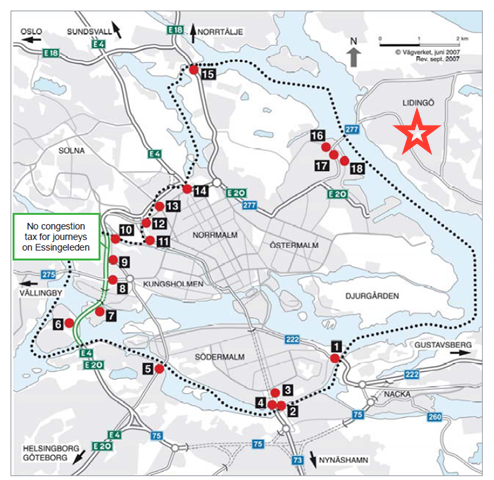
\includegraphics[width=5in]{../img/stockholm-map.png}
\caption{Stockholm Congestion Tax, access points in red. \citep{transportstyrelsen2015}}
\label{fig:stockholm-map}
\end{figure}

\begin{figure}
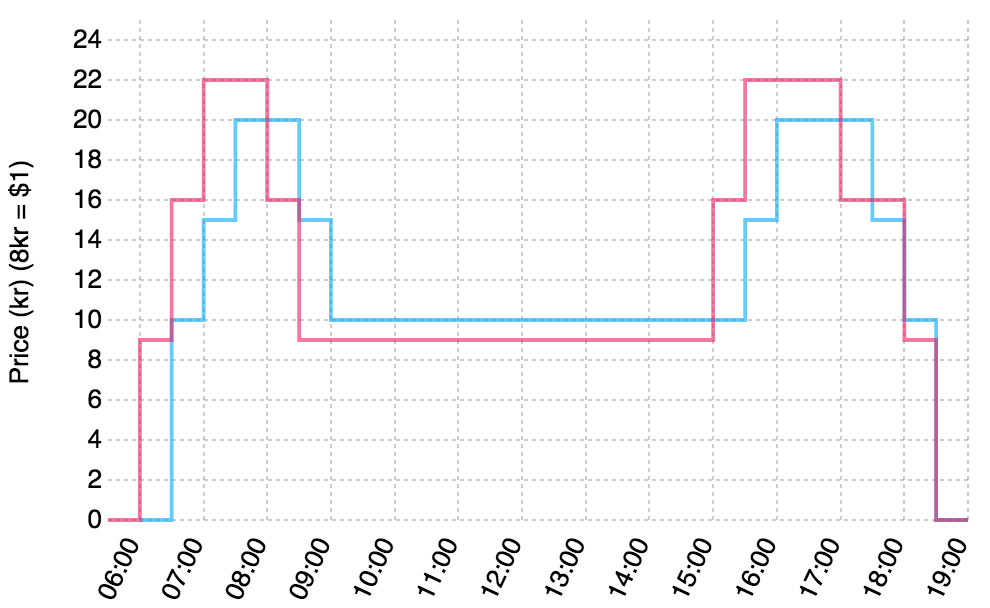
\includegraphics[width=4.5in]{../img/sweden-prices.png}
\caption{Sweden price structure \citep{transportstyrelsen2015}}
\label{fig:sweden-schedules}
\end{figure}


\subsection{Results}

The Tax has cut both traffic flow and travel times. Traversals of the cordon have fallen by 20-21\%. This figure was in excess of the forecast 16\% fall, due to the fact off-peak travel fell by almost the same amount (21\%) as peak travel (20\%) \citep{Eliasson2013}. Models had predicted off-peak travel would fall only 14\% due to lower mid-day charges. The fall in person-trips was similar for commuters (24\%) and discretionary travelers (22\%), but the two groups adapted differently: commuters who stopped driving switched to public transit, while discretionary travelers cancelled or rerouted their trips \citep{FranklinEtAl2010}. \citet{Eliasson2013} estimate that the Tax raised public transit ridership 4-5\%, or 8-10 thousand riders per day, and that vehicle-kilometers-traveled within the zone fell 10-15 percent. \citet{Karlstrom2009} find only weak evidence of departure time rescheduling.

\subsection{Finances}

The cost of the charging system trial was 1900 MSEK, of which 1050 MSEK was spent prior to charging \citep{Eliasson2009}. Another 1400 MSEK paid for the public transit expansion---mostly to buy 200 buses and run the extra services \citep[p. 398]{Eliason2008}. The literature agrees that design mistakes and politics inflated the 1900 MSEK, as explained in detail by \citet{Hamilton2011}. First, transaction costs for payment processing were originally high because every charge was processed as a separate bank transaction. Second, the Liding\"o exemption required an expensively low false negative rate (achieved by manually double-checking video), because if the system identifies a Liding\"o trip when it enters the cordon but misses it leaving (or vice versa), then it charges the exempt trip.\footnote{Jones Eliason, a researcher involved in the implementation, has remarked, ``Had we realized just how expensive the Liding\"o exception would be, it is unlikely that it would have been adopted'' \citep[p. 217]{Eliasson2009b}.} Third, delay caused by legal and political complications are estimated to have cost 600 MSEK \citep[p. 121]{GullbergIsaksson2009}. Fourth, spending on transponders and radio beacons were in some sense wasted. Finally, having such a short trial required expensive redundancy and overesign, because the system had to work perfectly and immediately with little testing.

Despite the challenging start, SCT has since turned out to be financial success: in 2008, operating costs were estimated to be 220 MSEK and revenues 710 MSEK, but by 2016 operating costs were down to 103 MSEK and revenues up to 1400 MSEK \citep[p. 40]{Borjesson2018}. 
